\documentclass[12pt, english]{article}
%%%%%%%%%%%%%%%%%%%%%%%%%%%%%%%%%%%%%%%%%%%%%%%%%%%%%%%%

% margin %%%%%%%%%%%%%%%%%%%%%%
\usepackage{geometry}
 \geometry{
 a4paper,
 left=1in,
 top=0.9in,
 right=1in,
 bottom=2in,
 }
%%%%%%%%%%%%%%%%%%%%%%%%%%%%%%%%%%%%%%%%%%%%%%%%%%%%%%%%

% page no. %%%%%%%%%%%%%%%%%%%%%%
\usepackage{fancyhdr}
\pagestyle{fancy}
\fancyhf{}
\fancyfoot[C]{\textit{\thepage}}
\setlength{\headheight}{65pt}
%%%%%%%%%%%%%%%%%%%%%%%%%%%%%%%%%%%%%%%%%%%%%%%%%%%%%%%%

% idk-needed %%%%%%%%%%%%%%%%%%%%%%
\usepackage{amsmath,amsthm,amssymb,amsfonts, enumitem, color, comment, graphicx, environ, lipsum, accsupp}
%%%%%%%%%%%%%%%%%%%%%%%%%%%%%%%%%%%%%%%%%%%%%%%%%%%%%%%%

% code and color %%%%%%%%%%%%%%%%%%%%%%
\usepackage{spverbatim}
\usepackage{xcolor}
\usepackage{listings}
\definecolor{bluegrey}{RGB}{0, 0, 200}
\lstset{
        framexleftmargin=0pt,
        frame=shadowbox,
        rulesepcolor=\color{gray},
        xleftmargin=30pt,
        xrightmargin=30pt,
        breaklines=true,
        basicstyle=\ttfamily,
        showstringspaces=false,
        escapeinside={(*@}{@*)},
        }
\def\speciallstcolor{\begingroup\color{blue}}
\def\endspeciallstcolor{\endgroup}
%%%%%%%%%%%%%%%%%%%%%%%%%%%%%%%%%%%%%%%%%%%%%%%%%%%%%%%%

% heading %%%%%%%%%%%%%%%%%%%%%%
\renewcommand\thesection{\color{blue}\arabic{section}}
\newcommand{\mysection}[2]{\setcounter{section}{#1}\addtocounter{section}{-1}\section{#2}}
%%%%%%%%%%%%%%%%%%%%%%%%%%%%%%%%%%%%%%%%%%%%%%%%%%%%%%%%

% image %%%%%%%%%%%%%%%%%%%%%%%
\graphicspath{}
%%%%%%%%%%%%%%%%%%%%%%%%%%%%%%%%%%%%%%%%%%%%%%%%%%%%%%%%

% both side indent %%%%%%%%%%%%%%%%%%%%%%
\newenvironment{myindent}
{\par\leftskip25pt\relax\rightskip25pt\relax}
{\par\leftskip0cm\relax\rightskip0cm\relax}
%%%%%%%%%%%%%%%%%%%%%%%%%%%%%%%%%%%%%%%%%%%%%%%%%%%%%%%%

% type ^ and \ %%%%%%%%%%%%%%%%%%%%%%
\newcommand{\power}{$^\wedge$}
\newcommand{\backs}{\textbackslash} 
%%%%%%%%%%%%%%%%%%%%%%%%%%%%%%%%%%%%%%%%%%%%%%%%%%%%%%%%

% document info %%%%%%%%%%%%%%%%%%%%%%
\lhead{Arav Sarma \\ 15193845}  %replace with your name
\rhead{Homework \textcolor{blue}{7} \\ 2025 Speech Processing}
%%%%%%%%%%%%%%%%%%%%%%%%%%%%%%%%%%%%%%%%%%%%%%%%%%%%%%%%

% begin %%%%%%%%%%%%%%%%%%%%%%
\begin{document}
%wwwwwwwwwwwwwwwwwwwwwwwwwwwwwwwwwwwwwwwwwwwwwwwwwwwwwwwww

% section _______________________________________________
\mysection{7}{Formants}
\vspace{10pt}
% -__-__-__-__-__-__-__-__-__-__-__-__-__-__-__-__-__-__-

% //////////////////////////////////////////////////////
\subsection*{\emph{1a.} Automating formant measurement} \vspace{15pt}

\begin{itemize}
    \item \textbf{Script} \vspace{5pt}
\begin{lstlisting}[xleftmargin=0pt,]
textgridFiles$# = fileNames$# ("sounds/*.TextGrid")
writeInfoLine: "Durations, pitches, and formants:"
for fileNumber to size (textgridFiles$#)
	textgridFile$ = textgridFiles$# [fileNumber]
	textgrid = Read from file: "sounds/" + textgridFile$
	numberOfIntervals = Get number of intervals: 1
	soundFile$ = textgridFile$ - ".TextGrid" + ".wav"
	sound = Read from file: "sounds/" + soundFile$
	pitchObject = To Pitch: 0, 75, 600
	selectObject: (*@\aftergroup\speciallstcolor@*)sound(*@\aftergroup\endspeciallstcolor@*)
	formantObject = To (*@\aftergroup\speciallstcolor@*)Formant (burg): 0, 5, 5000, 0.025, 50(*@\aftergroup\endspeciallstcolor@*)
	for interval to numberOfIntervals
		selectObject: textgrid
		text$ = Get label of interval: 1, interval
		if text$ = "v"
			startingTime = Get start time of interval: 1, interval
			endTime = Get end time of interval: 1, interval
			duration = endTime - startingTime
			selectObject: pitchObject
			pitch = Get mean: startingTime, endTime, "hertz"
			selectObject: (*@\aftergroup\speciallstcolor@*)formantObject(*@\aftergroup\endspeciallstcolor@*)
			f1 = (*@\aftergroup\speciallstcolor@*)Get quantile: 1, startingTime, endTime, "hertz", 0.5(*@\aftergroup\endspeciallstcolor@*)
			f2 = (*@\aftergroup\speciallstcolor@*)Get quantile: 2, startingTime, endTime, "hertz", 0.5(*@\aftergroup\endspeciallstcolor@*)
			appendInfoLine: "File ", textgridFile$ - ".TextGrid", ": ", " duration = ", fixed$ (duration, 3), " seconds,", " pitch = ", fixed$ (pitch, 3), " Hz,", " F1 = ", round (f1), " Hz, F2 = ", round (f2), " Hz."
		endif
	endfor
removeObject: (*@\aftergroup\speciallstcolor@*)textgrid, sound, pitchObject, formantObject(*@\aftergroup\endspeciallstcolor@*)
endfor
\end{lstlisting} \vspace{10pt}

    \item \textbf{Output} \vspace{5pt}
\begin{lstlisting}[xleftmargin=0pt]
Durations, pitches, and formants:
File ki-ba1:  duration = 0.060 seconds, pitch = 134.769 Hz, F1 = 273 Hz, F2 = 2065 Hz.
File ki-ba2:  duration = 0.075 seconds, pitch = 134.485 Hz, F1 = 273 Hz, F2 = 2087 Hz.
File ki-ba3:  duration = 0.090 seconds, pitch = 134.872 Hz, F1 = 274 Hz, F2 = 2216 Hz.
File kiba1:  duration = 0.032 seconds, pitch = 128.150 Hz, F1 = 284 Hz, F2 = 2153 Hz.
File kiba2:  duration = 0.039 seconds, pitch = 128.772 Hz, F1 = 281 Hz, F2 = 2126 Hz.
File kiba3:  duration = 0.055 seconds, pitch = 129.483 Hz, F1 = 280 Hz, F2 = 2040 Hz.
\end{lstlisting} \vspace{10pt}

\end{itemize}

% //////////////////////////////////////////////////////

% \\\\\\\\\\\\\\\\\\\\\\\\\\\\\\\\\\\\\\\\\\\\\\\\\\\\\\\\\\
\subsection*{\emph{1b.} Interpretation}

Average f1 is 273.3 Hz for short vowel and 281.7 for long vowels. Average f2 is 2106.3 Hz for short vowels, and 2122.6 Hz for long vowels. The formant differences between the two lengths are minute enough to consider them at the same vowel space. These slight differences do not influence perception of vowel length. This can answer why self-experiment in 5.2 did not result in perception of lengthened short vowel to be the same as original. This should hold true for the other way as well (shortened long vowel), however not enough tokens were tested in 5.2 to reach the phoneme boundary from the other side.

% \\\\\\\\\\\\\\\\\\\\\\\\\\\\\\\\\\\\\\\\\\\\\\\\\\\\\\\\\\

% \\\\\\\\\\\\\\\\\\\\\\\\\\\\\\\\\\\\\\\\\\\\\\\\\\\\\\\\\\
\subsection*{\emph{2d.} Filtering with formants}

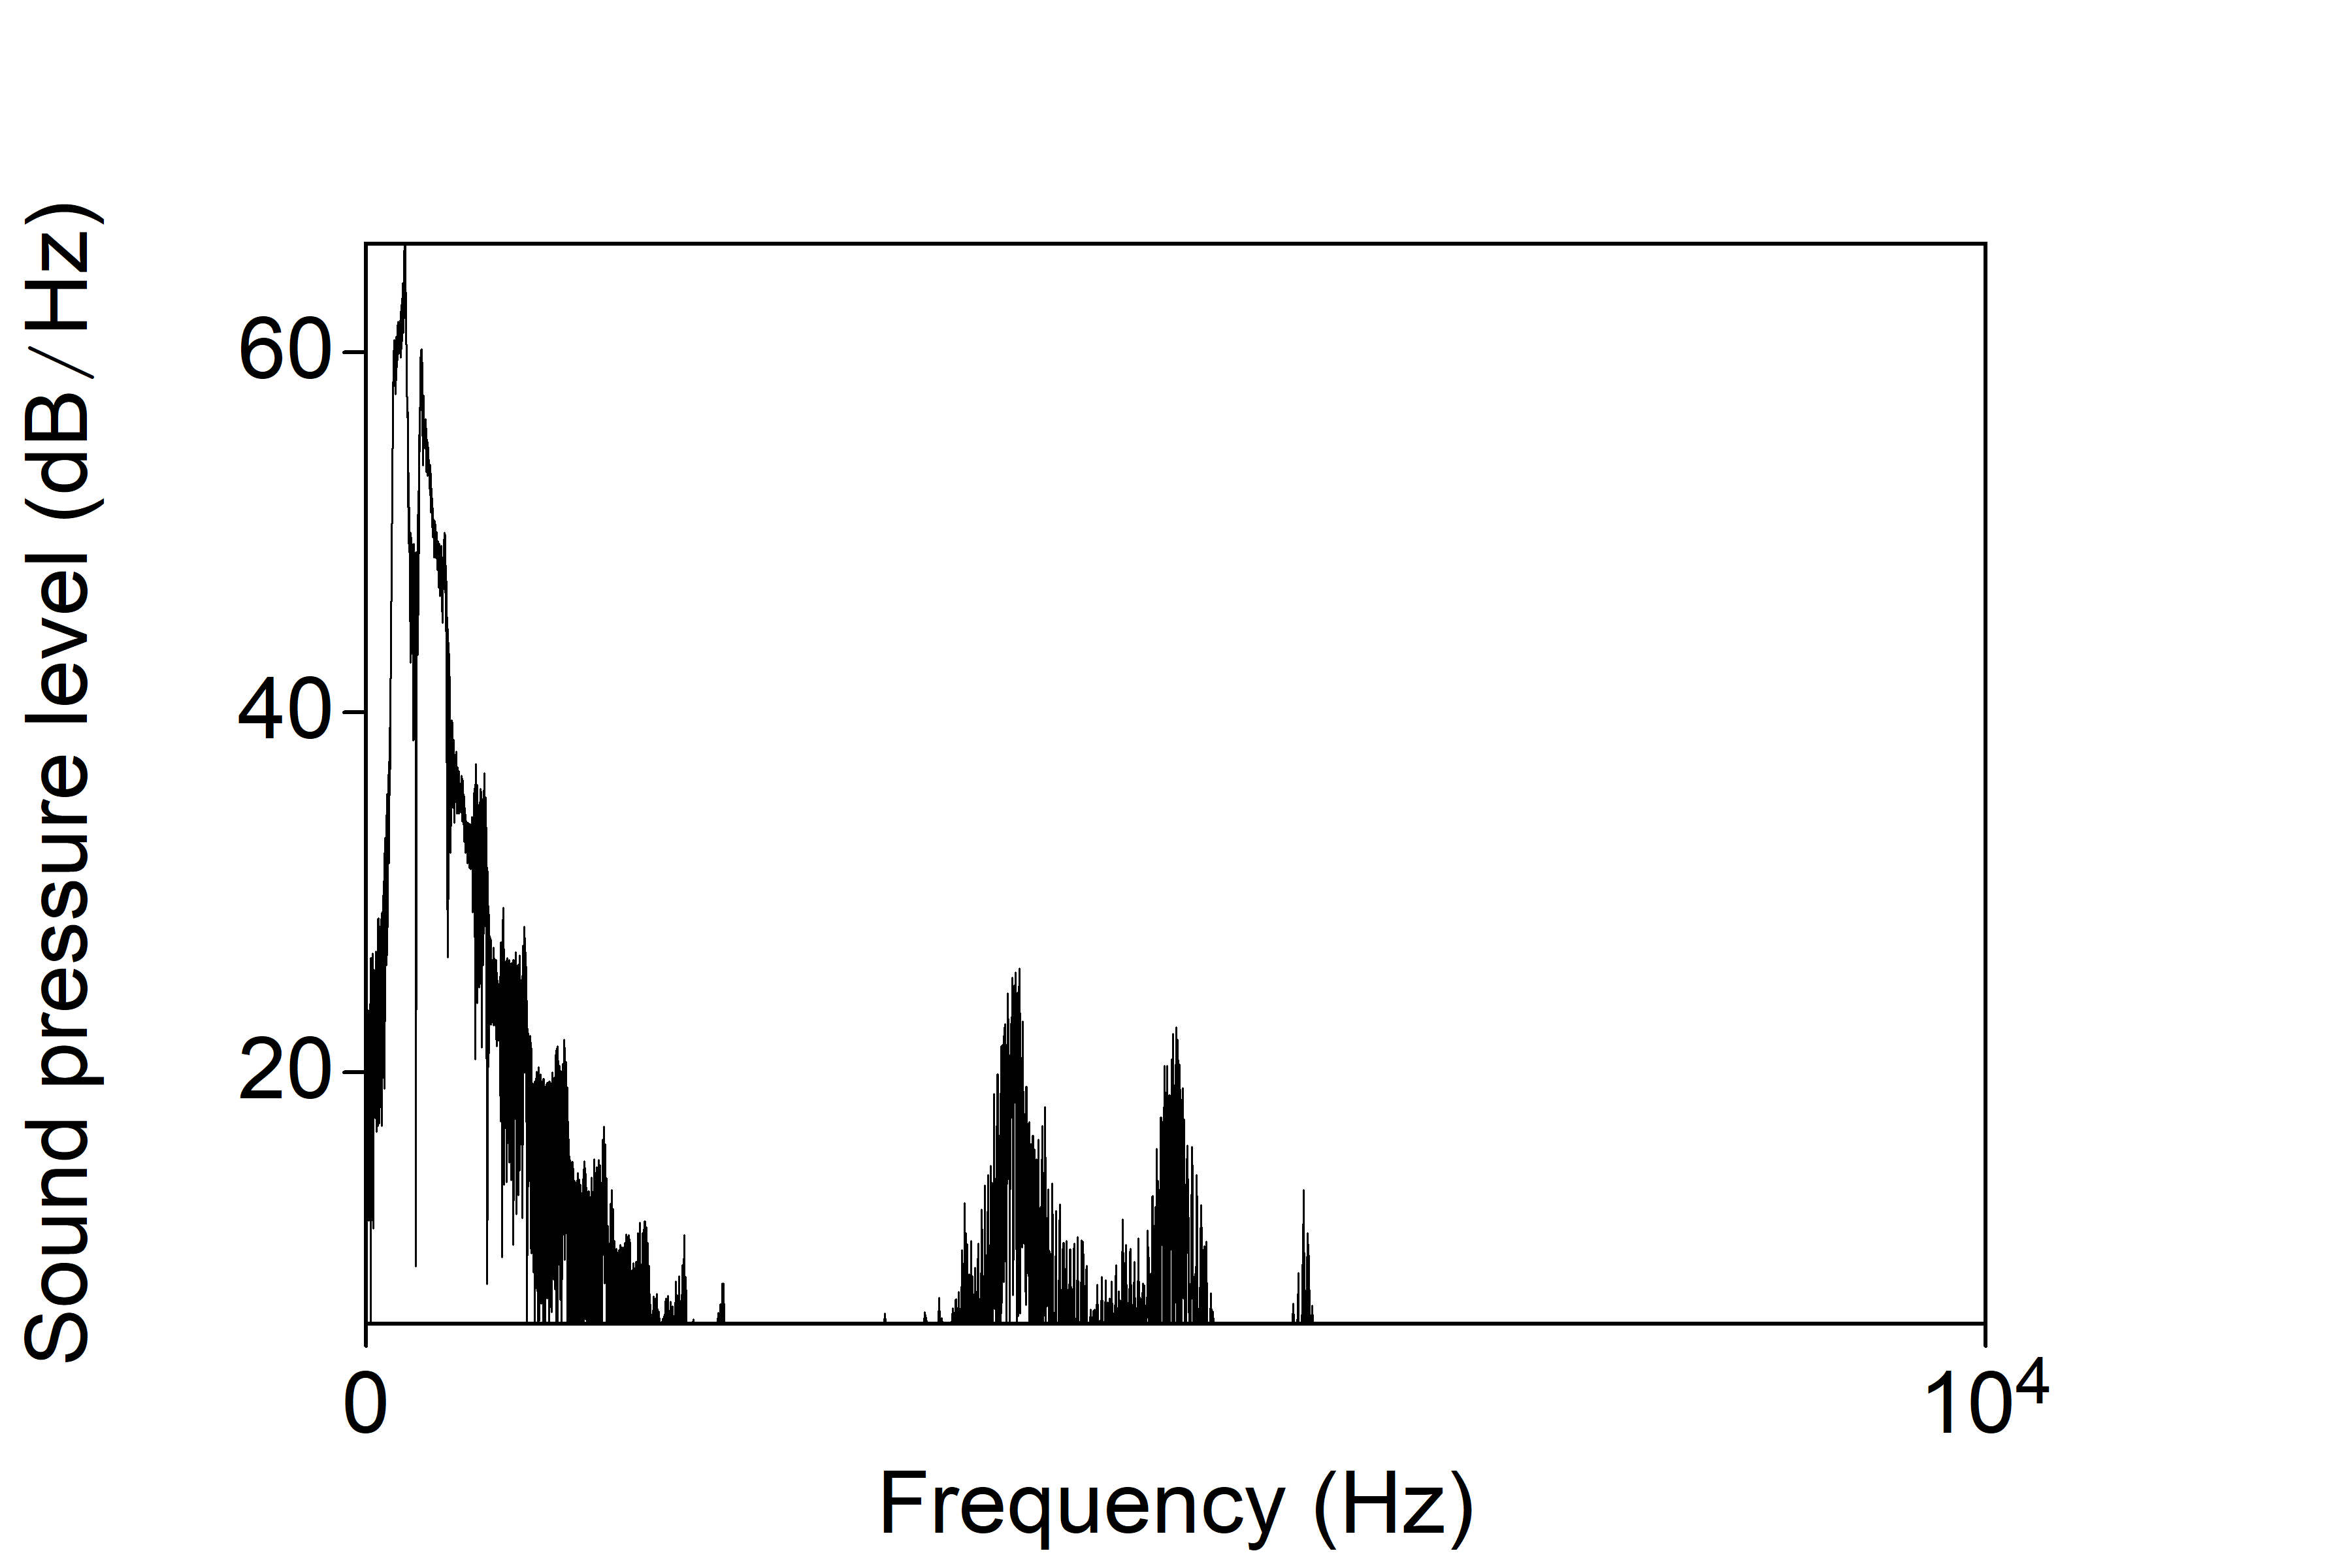
\includegraphics[]{f1345-spectrum.png}

% \\\\\\\\\\\\\\\\\\\\\\\\\\\\\\\\\\\\\\\\\\\\\\\\\\\\\\\\\\

\subsection*{\emph{2e.} The continuum} \vspace{15pt}

\begin{itemize}
    \item \textbf{Script} \vspace{5pt}
\begin{lstlisting}[xleftmargin=0pt,]
sound = Read from file: "source_F1_F3_F4_F5.wav"
for vowelNumber to 10
	f2 = 1250 + 125 * vowelNumber
	impulseResponse = Create Sound from formula: "F2", 1, 0.0, 0.05, 44100,
	... ~ sin (2*pi*f2*x) * 2^(-x/0.003)
	selectObject: sound, impulseResponse
	Convolve: "peak 0.99", "zero"
	Save as WAV file: "vowels/iu" + string$ (vowelNumber) + ".wav"
endfor
\end{lstlisting} \vspace{10pt}
\end{itemize}


% \\\\\\\\\\\\\\\\\\\\\\\\\\\\\\\\\\\\\\\\\\\\\\\\\\\\\\\\\\
\subsection*{\emph{2f.} Your classification of the continuum}

\begin{itemize}
    \item \textbf{iu1:} /u/
    \item \textbf{iu2-4ː} /ɯ/
    \item \textbf{iu5-8ː} /y/
    \item \textbf{iu8-10ː} /y/ or /i/ \par
    Going from iu1 to iu10, I hear most of them to be more u-like, and going through the other direction I tend to hear the iu10 as /i/ then rest as close to /u/ and all rounded. After going throught the sounds multiple times, I feel every other time I hear it differently. The robotic voice does not help.
\end{itemize}

% \\\\\\\\\\\\\\\\\\\\\\\\\\\\\\\\\\\\\\\\\\\\\\\\\\\\\\\\\\

% ><><><><><><><><><><><><><><><><><><><><><><><><><><><><><
\subsection*{\emph{3.} Formants and/or intensity in the acoustic continua of your experiment}
\vspace{10pt}

\begin{itemize}
    \item \textbf{General research question:} \par
    \textcolor{gray}{Location of phoneme boundary as a function of orthographic context (and exopure/familiarity with orthography of certain language(s))} \par
    \textbf{Location of phoneme boundary as a function of lexical context (word-nonword)}
    \item \textbf{\textcolor{gray}{Addition:}} \par
    \textcolor{gray}{L2 lexical knowledge context}
    \item \textbf{Specific research question:} \par
    \textcolor{gray}{My idea is to take both orthography and non-native lexical knowledge as a coupled effect on phonological categorisation. Preliminary thoughts on operationalising this question: looking at phonemic boundary between voiced-plain-aspirated, aspirated-fricative continua for L2 English speakers from Assam (or L1 Assamese speaking). Onset stop contrast on L2 variety is through voicing unlike aspiration in L1 English for Assamese (voicing+aspiration for Boro), Orthograhpic <b>, <d>, <g> are percieved as voiced like other Indian Englishes. This perception gets carried over even when exposed to L1 English. Questions: How much closure devoicing / afterburst duration can be blocked off during phoneme categorisation for a voicing / plain percept (how strong would lexical effect be on a word like `ban' / `pan', and also orthographic; eg: when shown <pan> / <phan or fan>)?} \par
    How does presence/absence of a lexical item effect categorisation of aspirated-breathy laryngeal contrast? Unlike the voicing or aspirated contrasts where boundary can be tested with VOT continua, the aspirated-breathy contrast would require manipulation of cues like turbulence quality and also pitch on following vowel (as the breathy and aspirated categories has been observed to effect pitch across languages; tonogenesis in Rohingya, Punjabi, tone-depressing effect in Southeastern Bantu, adaptation of indic loans with breathy in Thai). The study will look at lexical effect across this contrast for L1 Assamese speakers from Guwahati.       
    \item \textbf{Participants} \par
    Recruited: \char`\~ 7 \\
    Completed: 0 \par
    Participants are going to be tested online using Zoom online meetings, and recruited through author's contacts, and likely by reaching out to Assam/Northeast related online forums like on reddit. The plan is to have non-native English speakers ideally all from Guwahati with same L1, this is to neutralise individual factors like regional variation, exposure to English. A different experiment setup can be by using a qualtrics form along with online meet, so the participants have more autonomy with the test and excess to stimuli on their device while also making it easier to see if they are in a quiet environment. \par
    \item \textbf{Continua}
    Acoustic continua from [bha] to [pha]: 1st context is with following syllable [ŋa] (word to nonword). 2nd context is with following syllable [ki] (nonword to word). \\
    Continua from [dh] to [th]ː 1st context is with nucleus [ue] (word to nonword). 2nd context is with nucleus [io] (nonword to word). \par
    \item \textbf{Duration} \par
    The breathy-aspirated contrast can involve duration of voicing, however the breathy phonation is not really the same as voicing of a vowel (vocal folds in breathy are not as / or not completely close together as in modal voice). Therefore it is amount of voicing (closeness of vocal folds) during the afterburst which would be contrastive cue in terms of voicing. The other place where duration might be important is onset of vowel (duration of afterbust). However this will not be a cue used for this study's continua as it has not been investigated if it is involved in breathy-aspirated contrast and because onset of vowel is not easy to determine, especially if some amount of voicing is present before the vowe which can be the case for breathy phonemes.  \par
    \item \textbf{Pitch} \par
    Pitch is a cue which will be used to form continua. The vowel portion of the sound will be manipulated for gradient (mean) pitch. To synthesise different pitches, first the target pitch points in the manipulation window are selected, then they are scaled up/down to desired mean pitch via \textbf{Multiply pitch frequencies...}. \par
    Points to consider:
    \begin{itemize}
        \item How is pitch gradient incorporated with degree of voicing gradient: congruent + non-congruent?
    \end{itemize}
    \item \textbf{Intensity} \par
    Intensity of voicing is a likely cue which will be manipulated for the continua. The portion of the sound concerned for this manipulation is the afterburst (turbulent region between the burst and onset of vowel). To simulate a breathy-aspirated afterburst different ratios of periodicity to aperiodicity need to be synthesised. 
\end{itemize}
% ><><><><><><><><><><><><><><><><><><><><><><><><><><><><><

%wwwwwwwwwwwwwwwwwwwwwwwwwwwwwwwwwwwwwwwwwwwwwwwwwwwwwwwww
\end{document}